\documentclass[a4paper,12pt]{article}
\usepackage{mathrsfs}
\usepackage[utf8]{inputenc}
\usepackage[spanish]{babel}
\usepackage{amsmath}
\usepackage{amsfonts}
\usepackage{amssymb} 
\usepackage{graphicx} 
\usepackage{wrapfig}
\usepackage{enumitem}
\usepackage{fancyhdr}
\usepackage{float}
\usepackage{eurosym}
\usepackage{color}
\usepackage{circuitikz}
\usepackage{titling}
\usepackage{media9}
\usepackage{lipsum}
\usepackage{tocbibind}
\usepackage{listings}
\usepackage{tabularx}
\usepackage{tcolorbox}
\usepackage[table]{xcolor}
\usepackage{hyperref} 
\usepackage{bookmark}

\definecolor{lightblue}{RGB}{228, 244, 253}

\definecolor{dkgreen}{rgb}{0,0.6,0}
\definecolor{gray}{rgb}{0.5,0.5,0.5}
\definecolor{mauve}{rgb}{0.58,0,0.82}

\lstset{frame=tb,
  language=Python,
  inputencoding=utf8,
  extendedchars=true,
  aboveskip=3mm,
  belowskip=3mm,
  showstringspaces=false,
  columns=flexible,
  basicstyle={\small\ttfamily},
  numbers=none,
  numberstyle=\tiny\color{gray},
  keywordstyle=\color{blue},
  commentstyle=\color{dkgreen},
  stringstyle=\color{mauve},
  breaklines=true,
  breakatwhitespace=true,
  tabsize=3,
  literate=%
    {á}{{\'a}}1
    {é}{{\'e}}1
    {í}{{\'i}}1
    {ó}{{\'o}}1
    {ú}{{\'u}}1
    {ñ}{{\~n}}1
    {č}{{\v{c}}}1
}
\usepackage[left=3cm,right=3cm,top=3cm,bottom=4cm]{geometry}
\sloppy

% \pagestyle{fancy}
\providecommand{\abs}[1]{\lvert#1\rvert}
\providecommand{\norm}[1]{\lVert#1\rVert}

%%% Para las cabeceras
\newcommand{\hsp}{\hspace{20pt}}
\newcommand{\HRule}{\rule{\linewidth}{0.5mm}}
\headheight=50pt
%%% 
\newcommand{\vacio}{\textcolor{white}{ .}}

%%% Para que las ecuaciones se numeren
%%% con el número de sección y el de ecuación.
\renewcommand{\theequation}{\thesection.\arabic{equation}}


% Color azul para algunos 
% textos de la portada
\definecolor{azulportada}{rgb}{0.16, 0.32, 0.75}

%%%% Azul para textos de headings
\definecolor{azulinterior}{rgb}{0.0, 0.2, 0.6}

%%%%%%%%%%%%%%%%%%%%%%%%%%%%%%%%
%%%%%% Datos del proyecto %%%%%%
%%%%%%%%%%%%%%%%%%%%%%%%%%%%%%%%
%%%TÍTULO
%%% Escribirlo en minúsculas, el programa
%%% lo pondrá en mayúsculas en la portada.

\title{RL tabular sin modelo}

%%%% AUTORES
\author{Lydia Ruiz Martínez \and Pablo Tuñón Laguna \and Alberto Velasco Rodríguez}

%%%%%%%%%%%%%%%%%%%%%
%%%%%%%%%%%%%%%%%%%%
\begin{document}

%%%%%%%%%%%%%%%%%%%%%%%%%%%%%%%
%%%%%%%%%%%%%%%%%%%%%%%%%%%%%%%
\begin{titlepage} %%%%% Aquí no hay que tocar nada.
	%%%% Las siguientes instrucciones generarán automáticamente
	%%%% la portada de tu proyecto.
	%%% Cambio de la estructura de esta página
\thispagestyle{empty}
\newgeometry{left=0.6cm,top=1.2cm,bottom=1.2cm}

\fbox{\parbox[c]{18.5cm}{
\begin{center}
\vspace{1.5cm}
{\fontfamily{ptm}\fontsize{24}{28.8}\selectfont{Universidad Pontificia Comillas}}\\
[3.5em]
{\fontfamily{ptm}\fontsize{24}{5}\selectfont{ICAI}}\\
[3em]
{\fontfamily{ptm}\fontsize{28}{5}\selectfont{LABORATORIO 2}}\\
[1.5cm]
{\fontfamily{ptm}\fontsize{24}{5}\selectfont{Aprendizaje por refuerzo}}\\
[2cm]

% Autor del trabajo de investigación
\textcolor{azulportada}{\fontfamily{ptm}\fontsize{16}{5}\selectfont{\theauthor}}\\
[2cm]
% Título del trabajo
\textcolor{azulportada}
{\fontfamily{ptm}\fontsize{30}{5}\selectfont{\textsc{\thetitle}}}\\
%{\Huge\textbf{\thetitle}}\\
[1.2cm]

\includegraphics[width=8cm]{../fonts/Logo ICAI.png}
\\[1.8cm]

{\fontfamily{ptm}\fontsize{16}{5}\selectfont{Curso 2025-2026}}\\
[4cm]
\end{center}
}}
\restoregeometry
\end{titlepage}
 
 %%%% Volvemos a la estructura de la página normal

%%%%%%%%%%%%%%%%%%%%%%%%%%%%%%


%%%Encabezamiento y pie de página
%%% También se genera automáticamente
%%% Mejor no tocarlo mucho.
\renewcommand{\headrulewidth}{0.5pt}
\fancyhead[R]{
\textcolor{azulportada}{\fontfamily{ptm}\fontsize{10}{3}\selectfont{Lab 2 Aprendizaje por refuerzo}}\\
{\fontfamily{ptm}\fontsize{10}{3}\selectfont{\theauthor}}}
\fancyhead[L]{
  \textcolor{azulinterior}{\fontfamily{ptm}\fontsize{14}{4}\selectfont{\textbf{\thetitle}}}\\
}

\pagestyle{fancy}

\renewcommand{\footrulewidth}{0.5pt}
\fancyfoot[L]{\footnotesize Universidad Pontificia de Comillas (ICAI) --- curso 2025-2026}
\fancyfoot[C]{\vacio}
\fancyfoot[R]{\footnotesize Página \thepage}

%%%%%%%%%%%%%%%%%%%%

\renewcommand{\contentsname}{Índice}
\addtocontents{toc}{\protect\setcounter{tocdepth}{-1}} % Quita el índice de la tabla de contenidos
\tableofcontents
\addtocontents{toc}{\protect\setcounter{tocdepth}{2}}

\newpage


\section{Introducción}
En este informe se analiza la evolución y convergencia de los valores de acción \( Q(s, a) \) utilizando los algoritmos de aprendizaje por refuerzo \textbf{SARSA} y \textbf{Q-learning}. 
El estudio se centra en los estados \textbf{s13} y \textbf{s22}, evaluando la aproximación de los valores aprendidos a los valores óptimos obtenidos mediante \textit{Policy Iteration} (PI) y \textit{Value Iteration} (VI). 
Asimismo, se analiza el efecto de los hiperparámetros sobre la dinámica del aprendizaje.

%---------------------------
\section{SARSA}

\subsection{Implementación}
El algoritmo SARSA fue implementado respetando el esquema propuesto, actualizando los valores \( Q(s, a) \) siguiendo la política \(\epsilon\)-greedy. Las actualizaciones se realizan conforme a la siguiente ecuación:

\[
Q(s_t, a_t) \leftarrow Q(s_t, a_t) + \alpha \left[ r_{t+1} + \gamma Q(s_{t+1}, a_{t+1}) - Q(s_t, a_t) \right]
\]

\subsection{Convergencia de  Q(s, a)}

Se evalúa la convergencia de los siguientes pares estado-acción:

\begin{itemize}
    \item \( Q(13, \text{arriba-derecha}) \)
    \item \( Q(13, \text{abajo-derecha}) \)
    \item \( Q(22, \text{arriba-derecha}) \)
    \item \( Q(22, \text{abajo-derecha}) \)
\end{itemize}

Los valores obtenidos se comparan con los valores reales de Policy Iteration (PI) y Valure Iteration (VI):

\begin{table}[H]
    \centering
    \caption{Comparación de valores \( Q(s, a) \) en SARSA}
    \begin{tabular}{lccc}
        Estado-Acción & Valor SARSA & Valor Real (PI/VI) & Error Absoluto \\
        Q(13, ↑→) & 2.14 & 2.15 & 0.01 \\
        Q(13, ↓→) & 5.00 & 5.00 & 0.00 \\
        Q(22, ↑→) & 2.15 & 2.15 & 0.00 \\
        Q(22, ↓→) & -5.44 & -5.50 & 0.06 \\
    \end{tabular}
\end{table}
Se puede ver que el error acaba siendo ínfimo en los 4 pares, habiendo sólo dos pares que no consiguen un error de 0.
En concreto, estos pares son los de la acción menos desable para cada estado, debido a que la política $\epsilon$-greedy de comportamiento de Sarsa fomenta investigar más las opciones de máximo valor.

\subsection{Evolución de valores de Q}
En la figura 1 se puede observar que a partir del episodio 400 no aparecen apenas cambios en los valores de Q. Alcanzando ese error tan bajo alrededor a ese número de episodios. 
Además, llama la atención la variabilidad del par (22, ↑→) cuyo valor de Q cae por momentos.

\begin{figure}[H]
    \centering
    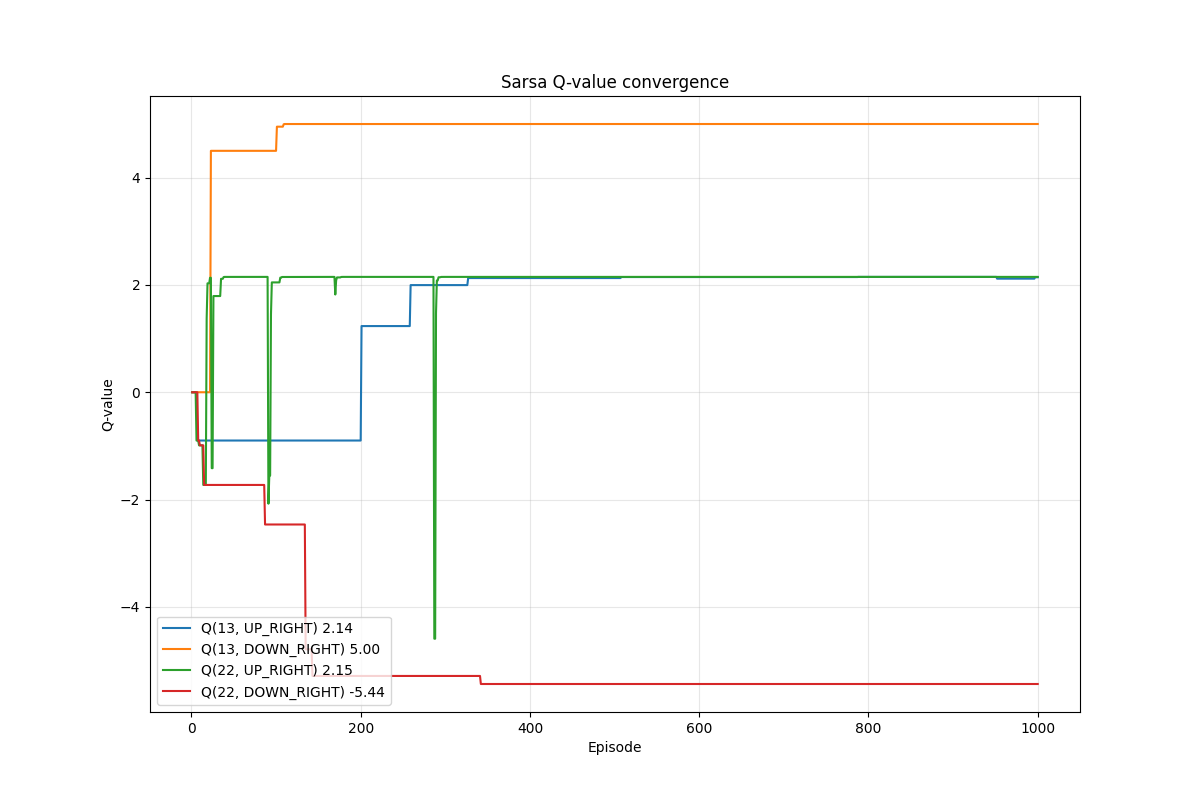
\includegraphics[width=0.7\textwidth]{../fonts/sarsa_q_convergence.png}
    \caption{Evolución de \( Q(s,a) \) con episodios (SARSA)}
\end{figure}

\subsection{Pasos medios por episodio}
En la figura 2 se puede ver que el número de episodios respecto al número de pasos forma prácticamente una recta. Aunque la pendiente va aumentando ligeramente, indicando que los episodios van durando menos pasos según se van completando. De hecho, la curva deja aumentar en pendiente a partir del episodio 400, debido a la covergencia de los valores de Q.
Podemos obtener el número de pasos medio que tarda en finalizar un episodio con el número total de pasos entre el número de episodios, lo cual es aproximadamente 3000/1000 = 3.
\begin{figure}[H]
    \centering
    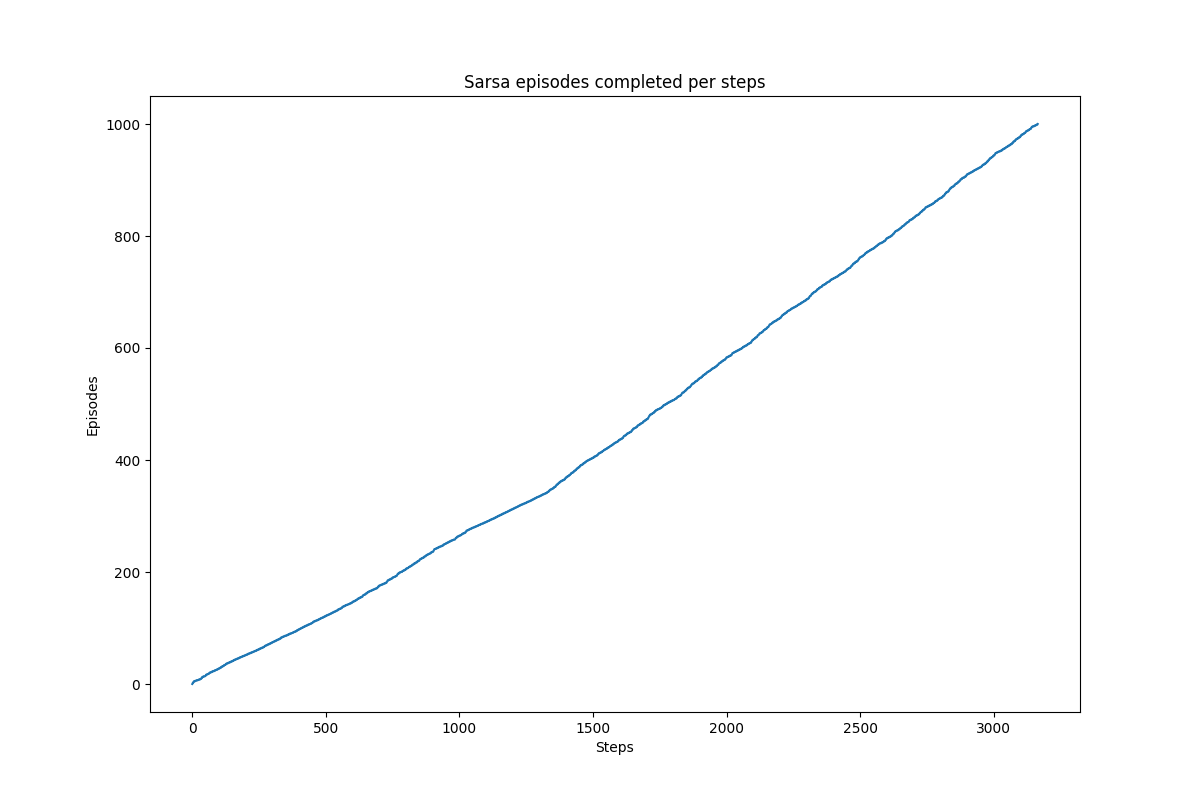
\includegraphics[width=0.5\textwidth]{../fonts/sarsa_steps_eps_2.png}
    \caption{Episodios exitosos vs pasos (SARSA)}
\end{figure}

%---------------------------
\clearpage
\section{Q-learning}

\subsection{Implementación}
El algoritmo Q-learning se implementó en el archivo \texttt{q\_learning.py}. 
A diferencia de SARSA, Q-learning actualiza \( Q(s, a) \) utilizando la acción con el valor máximo en el siguiente estado:

\[
Q(s_t, a_t) \leftarrow Q(s_t, a_t) + \alpha \left[ r_{t+1} + \gamma \max_{a'} Q(s_{t+1}, a') - Q(s_t, a_t) \right]
\]

\subsection{Convergencia de Q(s, a)}

Se evaluaron los mismos pares estado-acción que en SARSA.

\begin{table}[H]
    \centering
    \caption{Comparación de valores \( Q(s, a) \) en Q-learning}
    \begin{tabular}{lccc}
        Estado-Acción & Valor Q-learning & Valor Real (PI/VI) & Error Absoluto \\
        Q(13, ↑→) & 1.52 & 2.15 & 0.63 \\
        Q(13, ↓→) & 5.00 & 5.00 & 0.00 \\
        Q(22, ↑→) & 2.15 & 2.15 & 0.00 \\
        Q(22, ↓→) & -5.50 & -5.50 & 0.00 \\
    \end{tabular}
\end{table}
Se obtiene un error de 0 en 3 de los pares. Sin embargo, el par (13, ↑→) obtiene un error de 0.63, mucho mayor a cualquiera obtenido con SARSA. 
Al igual que en SARSA, sólo se obtiene error en el caso de la acción menos deseable.
\subsection{Evolución de valores de Q}

\begin{figure}[H]
    \centering
    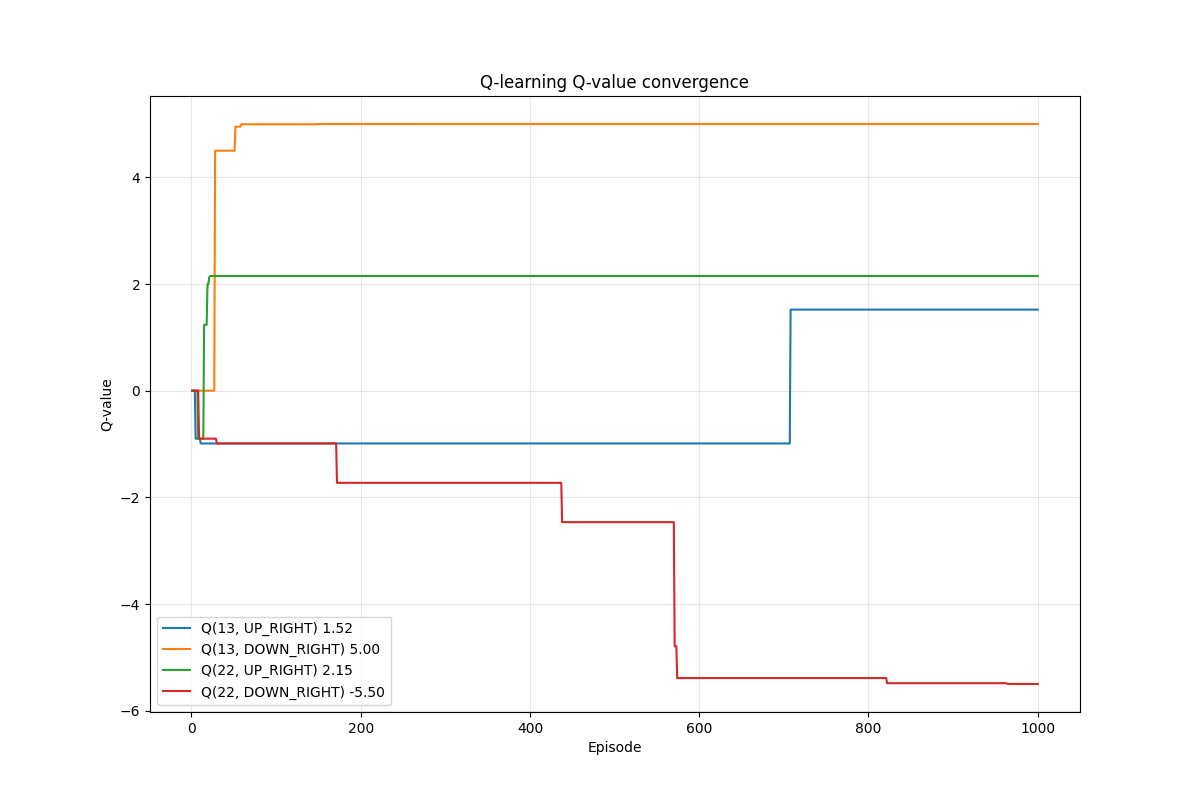
\includegraphics[width=0.75\textwidth]{../fonts/q_learning_q_convergence.png}
    \caption{Evolución de \( Q(s,a) \) con episodios (Q-learning)}
\end{figure}
En la figura 3 se puede observar que Q-learning es más estable que SARSA. Además, los valores de Q para las acciones más deseables convergen muy rápidamente al valor real. 
Por otro lado, el valor de Q para las acciones menos deseables tarda bastante en converger (800 episodios). 

\subsection{Pasos medios por episodio}
En la figura 4 podemos ver que el número de episodios exitosos respecto al número de pasos forma una recta de pendiente 4300/1000 = 4.3. Con Q-learning los episodios duran bastante más que con SARSA. Al tomar la acción con mayor Q se evita explorar opciones que a priori parecen peores, pero que pueden resultar mejores. Un ejemplo de esto es preferir acabar el episodio cuanto antes, porque intentar llegar al estado 19 acaba incurriendo en una mayor pérdida, algo que Q-learning tiende a no ver.

\begin{figure}[H]
    \centering
    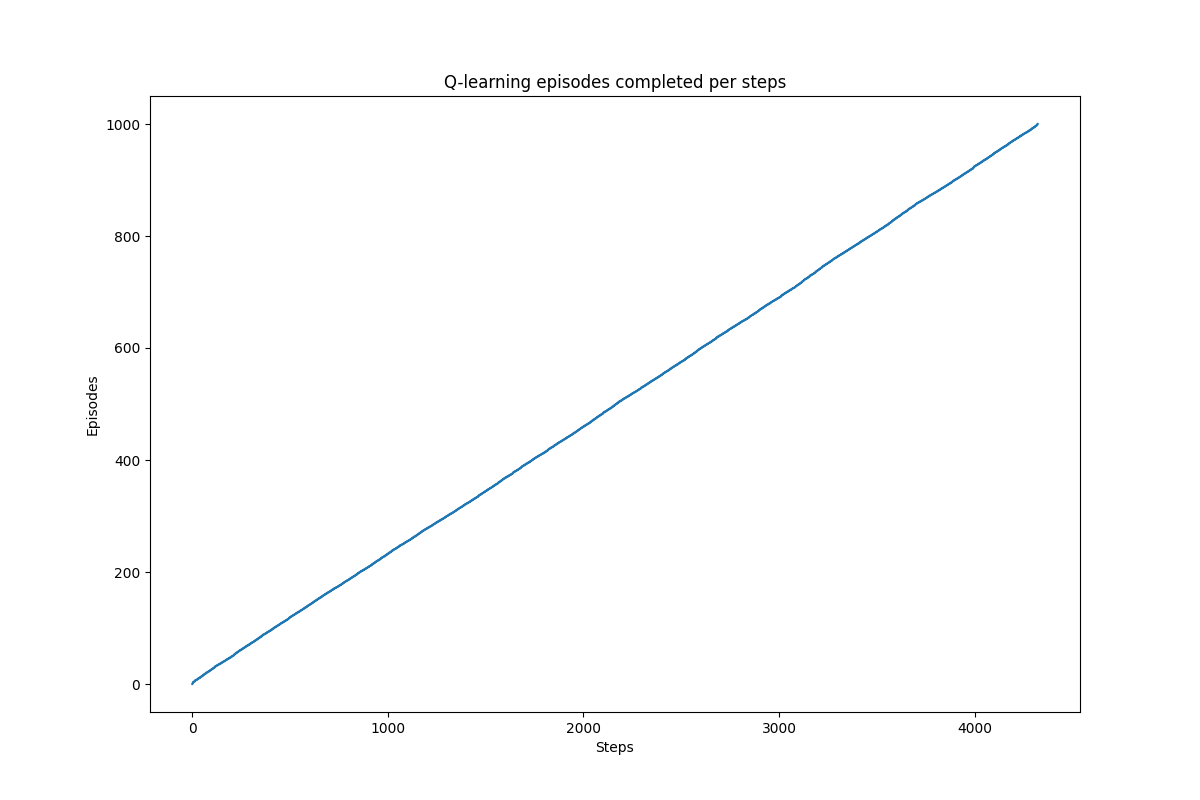
\includegraphics[width=0.75\textwidth]{../fonts/q_learning_steps_eps_2.png}
    \caption{Episodios exitosos vs pasos (Q-learning)}
\end{figure}

%---------------------------
\clearpage
\section{Comparación entre SARSA y Q-learning}

\begin{table}[H]
    \centering
    \caption{Comparación de desempeño}
    \begin{tabular}{lcc}
        Métrica & SARSA & Q-learning \\
        Velocidad de convergencia & 400 & 800 \\
        Velocidad de convergencia (acción óptima "clara") & 200 & 100 \\
        Exploración & Mejor & Peor \\
        Error final & 0.07 & 0.063 \\
    \end{tabular}
\end{table}

\subsection*{Observaciones}

\begin{itemize}
    \item SARSA mostró una convergencia más rápida para el global de los valores.
    \item Q-learning obtuvo una convergencia más rápida para los valores de Q de la acción óptima de estados donde se debe intentar maximizar el valor a corto plazo.
\end{itemize}

%---------------------------
\section{Conclusiones}

Ambos algoritmos logran aproximar los valores óptimos de Q(s, a) dados suficientes episodios. Para estados donde la acción según el valor a largo plazo difiere de la acción según el valor a corto plazo Q-learning lo puede tener complicado. Esto es dado que Q-learning tarda más en refinar los valores de Q para las acciones que no son preferibles a primera vista. Mietras tanto SARSA tarda menos en converger en general. Esta comparativa muestra los problemas de Q-learning y las ventajas de doble Q-learning para protegerse frente a acciones aparentemente buenas que a largo plazo no lo son.


\end{document}



